%%%%%%%%%%%%%%%%%%%%%%%%%%%%%%%%%%%%%%%%%%%%%%%%%%%%%%%%%%%%%%%%%%%%%%%%%%%%%%%%%%%%%%%%%%%%%%%%%%%%%%%%%%%%%%%%%%%%%%%%%%%%%%%%%%%%%%%%%%%%%%%%%%%%%%%%%%%%%%%%%%%
% Written By Michael Brodskiy
% Class: Fundamentals of Electromagnetics
% Professor: E. Marengo Fuentes
%%%%%%%%%%%%%%%%%%%%%%%%%%%%%%%%%%%%%%%%%%%%%%%%%%%%%%%%%%%%%%%%%%%%%%%%%%%%%%%%%%%%%%%%%%%%%%%%%%%%%%%%%%%%%%%%%%%%%%%%%%%%%%%%%%%%%%%%%%%%%%%%%%%%%%%%%%%%%%%%%%%

\documentclass[12pt]{article} 
\usepackage{alphalph}
\usepackage[utf8]{inputenc}
\usepackage[russian,english]{babel}
\usepackage{titling}
\usepackage{amsmath}
\usepackage{graphicx}
\usepackage{enumitem}
\usepackage{amssymb}
\usepackage[super]{nth}
\usepackage{everysel}
\usepackage{ragged2e}
\usepackage{geometry}
\usepackage{multicol}
\usepackage{fancyhdr}
\usepackage{cancel}
\usepackage{siunitx}
\usepackage{physics}
\usepackage{tikz}
\usepackage{mathdots}
\usepackage{yhmath}
\usepackage{cancel}
\usepackage{color}
\usepackage{array}
\usepackage{multirow}
\usepackage{gensymb}
\usepackage{tabularx}
\usepackage{extarrows}
\usepackage{booktabs}
\usepackage{lastpage}
\usepackage{float}
\usetikzlibrary{fadings}
\usetikzlibrary{patterns}
\usetikzlibrary{shadows.blur}
\usetikzlibrary{shapes}

\geometry{top=1.0in,bottom=1.0in,left=1.0in,right=1.0in}
\newcommand{\subtitle}[1]{%
  \posttitle{%
    \par\end{center}
    \begin{center}\large#1\end{center}
    \vskip0.5em}%

}
\usepackage{hyperref}
\hypersetup{
colorlinks=true,
linkcolor=blue,
filecolor=magenta,      
urlcolor=blue,
citecolor=blue,
}


\title{Final Exam}
\date{December 12, 2023}
\author{Michael Brodskiy\\ \small Professor: E. Marengo Fuentes}

\begin{document}

\maketitle

\begin{enumerate}

  \item 

    \begin{enumerate}

      \item 

        We know that, with a Hertzian dipole antenna centered at the origin, we may express the phasor as (as per eq. 9.44a):

        $$\boxed{\tilde{E}_\theta=60jI_o\left[ \frac{\cos\left( \frac{\pi}{2}\cos(\theta) \right)}{\sin(\theta)} \right]\left( \frac{e^{-jkR}}{R} \right)}$$

      \item 

        We know that the resistance as perceive by the transmission line may be written as:

        $$R_{in}=R_{rad}+R_{loss}$$

        A half-wave dipole means that $R_{loss}<<R_{rad}$, which allows us to approximate:

        $$R_{in}\approx R_{rad}$$

        Using equation 9.33a, we may write:

        $$R_{in}\approx\frac{2P_{rad}}{I_o^2}$$

        Using our answer from (d), we write:

        $$R_{in}\approx 2(36.57)$$
        $$R_{in}=73.14[\si{\ohm}]$$

        As stated in the textbook, for a half-wave dipole, the impedance is approximately $42[\si{\ohm}]$, which yields:

        $$\boxed{Z_{in}=73.14+42j[\si{\ohm}]}$$

        Note: the complex term can go to zero with a very slight change in dipole length, so we may simply write:

        $$\boxed{Z_{in}=73.14[\si{\ohm}]}$$

      \item 

        To match the impedance with no reflection, we want the reflection coefficient to be 0. Thus, we may write the reflection coefficient as:

        $$\Gamma=\frac{Z_L-Z_0}{Z_L+Z_0}$$

        Since we want no reflection, $\Gamma\to0$, which gives us:

        $$Z_L-Z_0=0$$

        Thus, to match with no reflection, we want to create a system such that $Z_L=Z_0$, which would mean:

        $$\boxed{Z_0=73.14+42j[\si{\ohm}]}$$

        Or, if we drop the complex term:

        $$\boxed{Z_0=73.14[\si{\ohm}]}$$


      \item 

        We know the radiated power may be found by integrating the real part of:

        $$dP_{rad}=R^2S(R,\theta,\phi)\,d\omega$$

        Which is the Poynting vector. Thus, we write:

        $$P_{rad}=\int\int \frac{R^2}{2\eta_o}\tilde{E}_\theta^2\,d\Omega$$

        This gives us:

        $$P_{rad}=\frac{15I_o^2}{\pi}\int\int\left[ \frac{\cos\left( \frac{\pi}{2}\cos(\theta) \right)}{\sin(\theta)} \right]^2\,d\Omega$$
        $$P_{rad}=\frac{15I_o^2}{\pi}\int\int\left[ \frac{\cos\left( \frac{\pi}{2}\cos(\theta) \right)}{\sin(\theta)} \right]^2\sin(\theta)\,d\theta\,d\phi$$
        $$P_{rad}=\frac{15I_o^2}{\pi}\int_0^{2\pi}\int_0^\pi\left[ \frac{\cos^2\left( \frac{\pi}{2}\cos(\theta) \right)}{\sin(\theta)} \right]\,d\theta\,d\phi$$
        $$P_{rad}=\frac{15I_o^2}{\pi}\left(2\pi  \right)\left( 1.219 \right)$$

        Substituting our value for $I_o$, we get:

        $$\boxed{P_{rad}=36.57[\si{\watt}]}$$

      \item 

        We want the equation to shift such that $R\prime$ is the new radius, which depends on $R$, $\theta$, and $h$. We know the parametrization of spherical coordinates may be written as:

        $$x=r\sin(\theta)\cos(\phi)$$
        $$y=r\sin(\theta)\sin(\phi)$$
        $$z=r\cos(\theta)$$

        We can substitute $R$ from (a) such that $R\to\sqrt{x^z+y^2+z^2}$:

        $$\tilde{E}_\theta=60jI_o\left[ \frac{\cos\left( \frac{\pi}{2}\cos(\theta) \right)}{\sin(\theta)} \right]\left( \frac{e^{-jk\sqrt{x^2+y^2+z^2}}}{\sqrt{x^2+y^2+z^2}} \right)$$

        We know that the shift in $x$ will lead to $x\to x-h$:

        $$\tilde{E}_\theta=60jI_o\left[ \frac{\cos\left( \frac{\pi}{2}\cos(\theta) \right)}{\sin(\theta)} \right]\left( \frac{e^{-jk\sqrt{(x-h)^2+y^2+z^2}}}{\sqrt{(x-h)^2+y^2+z^2}} \right)$$

        Combining the above with the parametrization, we get:

        $$\tilde{E}_\theta=60jI_o\left[ \frac{\cos\left( \frac{\pi}{2}\cos(\theta) \right)}{\sin(\theta)} \right]\left( \frac{e^{-jk\sqrt{(R\sin(\theta)\cos(\phi)-h)^2+(R\sin(\theta)\sin(\phi))^2+(R\cos(\theta))^2}}}{\sqrt{(R\sin(\theta)\cos(\phi)-h)^2+(R\sin(\theta)\sin(\phi))^2+(R\cos(\theta))^2}} \right)$$

        We can simplify this a bit to get:

        $$\boxed{\tilde{E}_\theta=60jI_o\left[ \frac{\cos\left( \frac{\pi}{2}\cos(\theta) \right)}{\sin(\theta)} \right]\left( \frac{e^{-jk\sqrt{R^2-2hR\sin(\theta)\cos(\phi)+h^2}}}{\sqrt{R^2-2hR\sin(\theta)\cos(\phi)+h^2}} \right)}$$

      \item 

        The PEC will produce some reflection such that we can write:

        $$\tilde{E}_\theta^i+\tilde{E}_\theta^r=\tilde{E}_\theta^t$$

        The reflected term, $\tilde{E}_\theta^r$, can be defined similar to how we defined the $h$-shifted antenna, except that we add the $h$ (picture this as a two-antenna array, with both $h$ away):

        $$\tilde{E}_\theta^r=60jI_o\left[ \frac{\cos\left( \frac{\pi}{2}\cos(\theta) \right)}{\sin(\theta)} \right]\left( \frac{e^{-jk\sqrt{R^2+2hR\sin(\theta)\cos(\phi)+h^2}}}{\sqrt{R^2+2hR\sin(\theta)\cos(\phi)+h^2}} \right)$$

        For ease of reading, let us assign two variables such that:

        $$a=\sqrt{R^2-2hR\sin(\theta)\cos(\phi)+h^2}$$

        and 

        $$b=\sqrt{R^2+2hR\sin(\theta)\cos(\phi)+h^2}$$

        From here, the total electric field may be computed as:

        $$\boxed{\tilde{E}_\theta^t=60jI_o\left[ \frac{\cos\left( \frac{\pi}{2}\cos(\theta) \right)}{\sin(\theta)} \right]\left( \frac{e^{-jka}}{a}-\frac{e^{-jkb}}{b} \right)}$$

      \item 

        The plots generated look as follows:

        \begin{figure}[H] \centering
          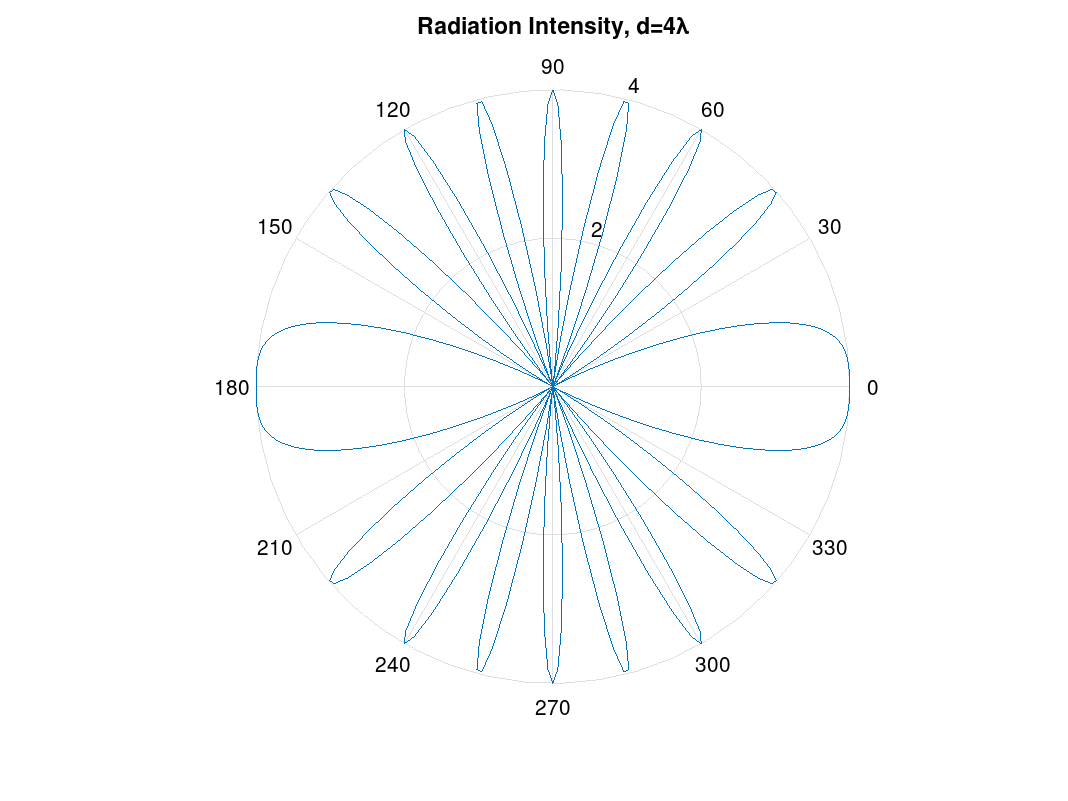
\includegraphics[width=.7\textwidth]{Figures/4lambda.png}
          \caption{Figure for $h=4\lambda$}
          \label{fig:1}
        \end{figure}

        \begin{figure}[H]
          \centering
          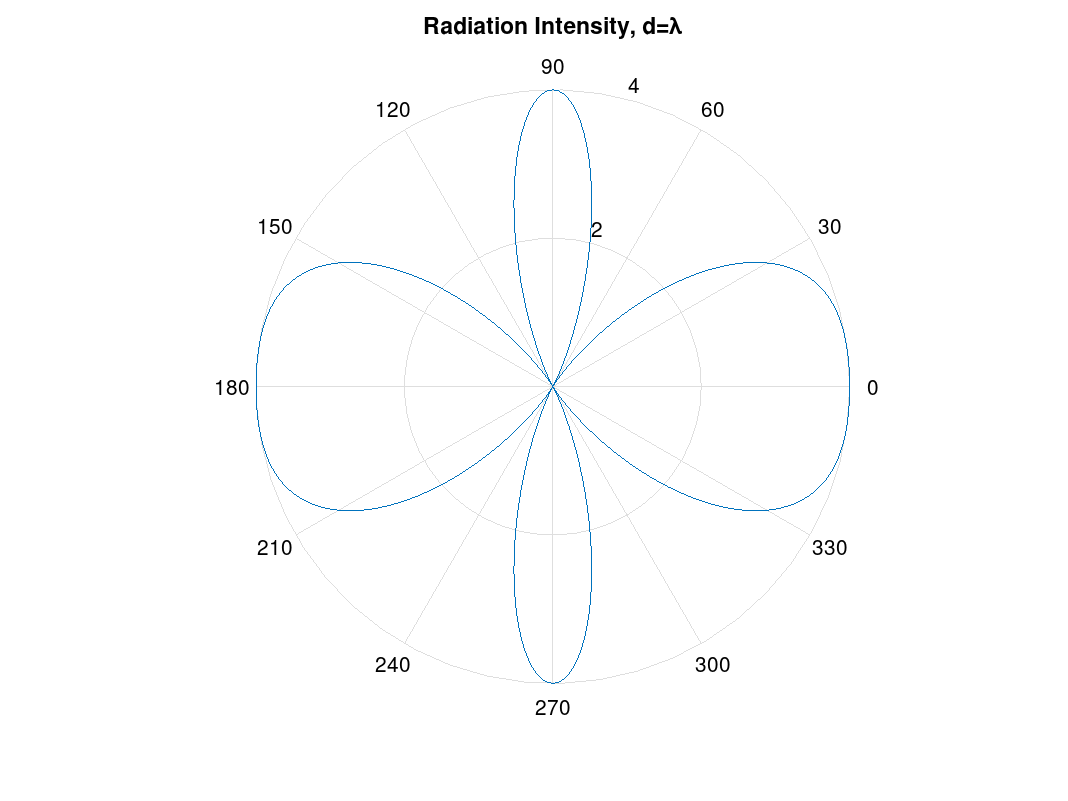
\includegraphics[width=.7\textwidth]{Figures/lambda.png}
          \caption{Figure for $h=\lambda$}
          \label{fig:2}
        \end{figure}

        \begin{figure}[H]
          \centering
          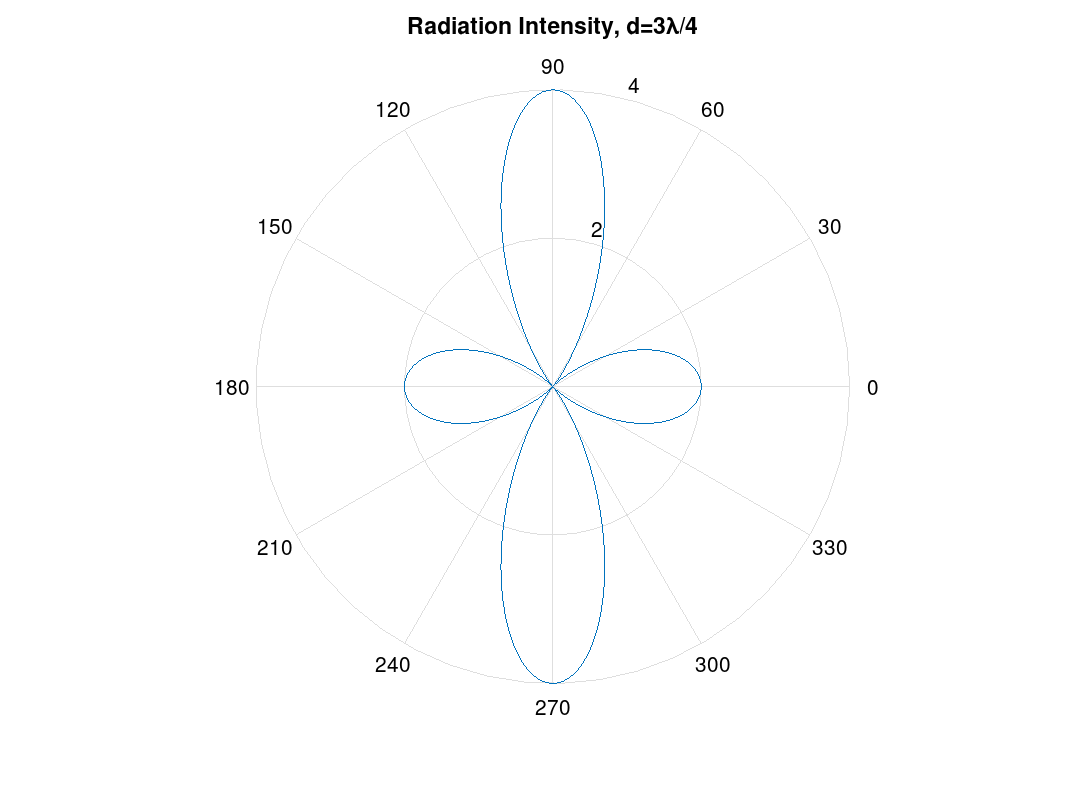
\includegraphics[width=.7\textwidth]{Figures/3lambda-4.png}
          \caption{Figure for $h=.75\lambda$}
          \label{fig:3}
        \end{figure}

        \begin{figure}[H]
          \centering
          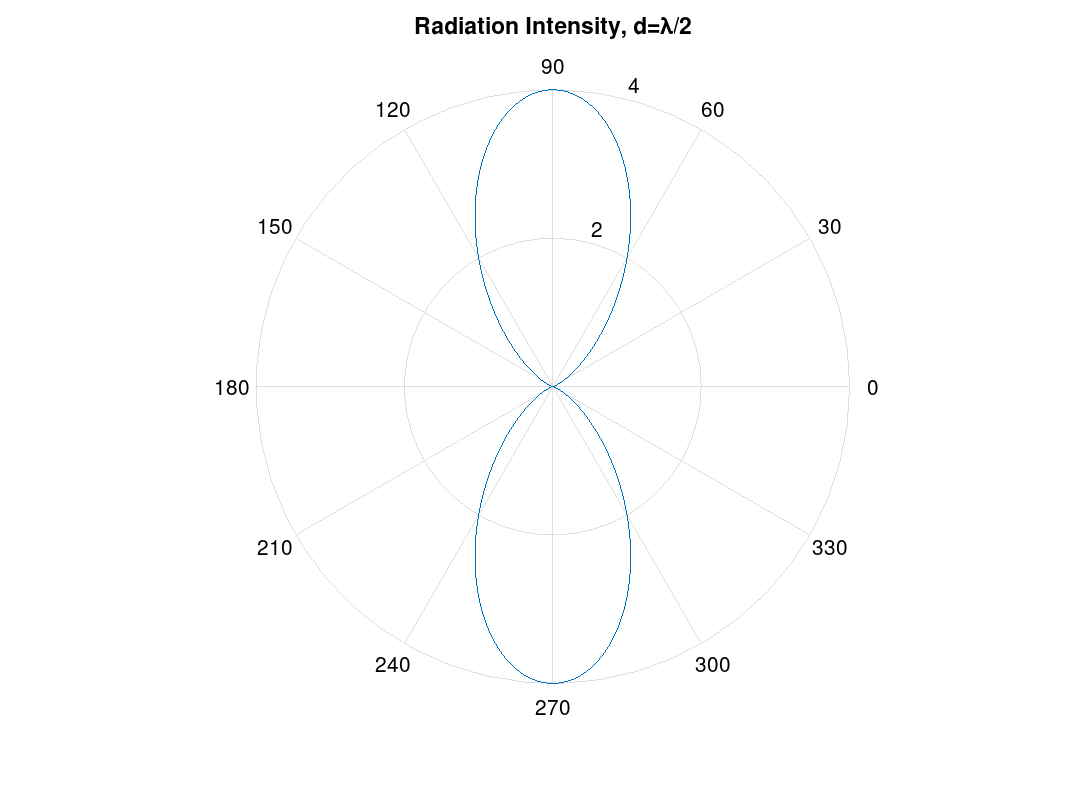
\includegraphics[width=.7\textwidth]{Figures/lambda-2.png}
          \caption{Figure for $h=.5\lambda$}
          \label{fig:4}
        \end{figure}

        \begin{figure}[H]
          \centering
          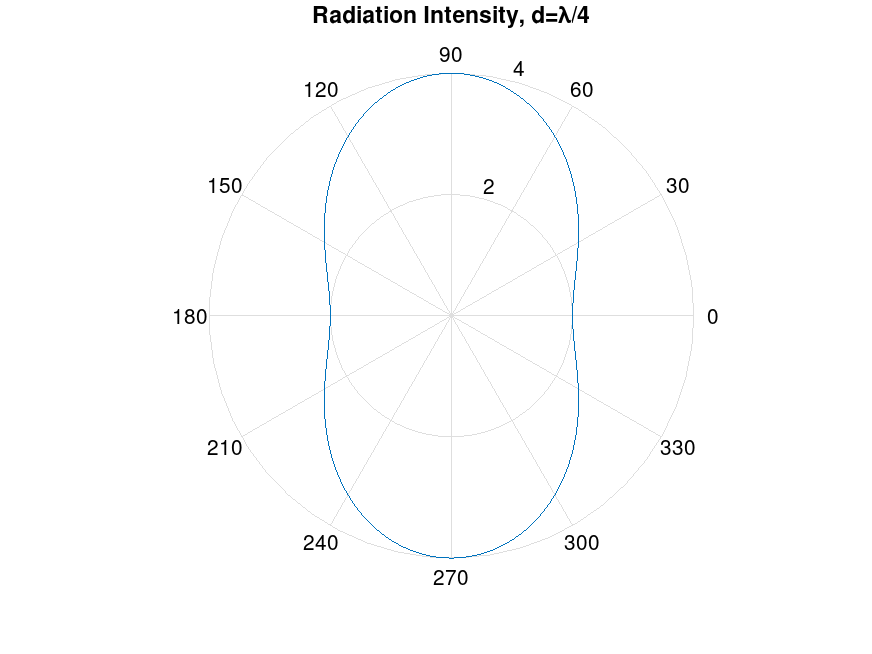
\includegraphics[width=.7\textwidth]{Figures/lambda-4.png}
          \caption{Figure for $h=.25\lambda$}
          \label{fig:5}
        \end{figure}

      \item 

        The PEC will produce some reflection such that we can write:

        $$\tilde{E}_\theta^i+\tilde{E}_\theta^r=\tilde{E}_\theta^t$$

        This time, we can imagine a reflected antenna shifted $-4\lambda$ and $-h$. Thus, we can get:

        $$c\to\sqrt{(R\sin(\theta)\cos(\phi)-h)^2+(R\sin(\theta)\sin(\phi))^2+(R\cos(\theta)-4\lambda)^2}$$
        $$c\to\sqrt{R^2-2hR\sin(\theta)\cos(\phi)-8\lambda R\cos(\theta)+h^2+16\lambda^2}$$

        $$\tilde{E}_\theta^r=60jI_o\left[ \frac{\cos\left( \frac{\pi}{2}\cos(\theta) \right)}{\sin(\theta)} \right]\left( \frac{e^{-jkc}}{c} \right)$$

        The total electric fields thus becomes:

        $$\tilde{E}_\theta^t=60jI_o\left[ \frac{\cos\left( \frac{\pi}{2}\cos(\theta) \right)}{\sin(\theta)} \right]\left( \frac{e^{-jka}}{a}+\frac{e^{-jkc}}{c} \right)$$

      \item See Plots Below

        \begin{figure}[H]
          \centering
          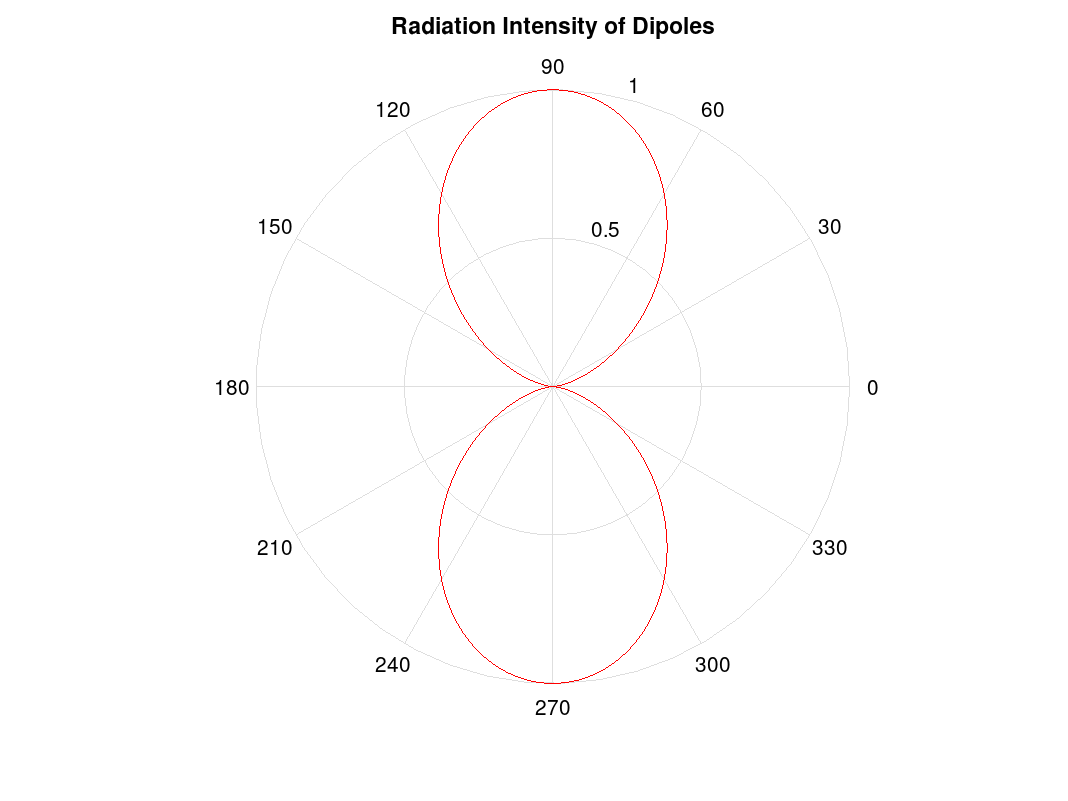
\includegraphics[width=.7\textwidth]{Figures/RI.png}
          \caption{Radiation Intensity Plots}
          \label{fig:6}
        \end{figure}

    \end{enumerate}

  \item 

        We know that, for an array consisting of two antennas, we may write the array factor as:

        $$AF_2=4\cos^2\left[ \frac{\pi}{\lambda}d\cos(\theta)+\frac{\phi}{2} \right]$$

        with $\beta$ as the wave number.

    \begin{enumerate}

      \item 

        Given that there is no phase difference, we may write (using the above equation):

        $$AF_2=4\cos^2\left[ \frac{\pi d}{\lambda}\cos(\theta) \right]$$

        We are asked to find an angle $\theta$ such that there is a maximum at:

        $$\theta=30$$

        Plugging this into our equation, we may write:

        $$AF_2=4\cos^2\left(\frac{\pi d\sqrt{3}}{2\lambda}\right)$$

        We know that the $\cos$ term will be at a maximum when the inside is an integer ($n$) multiple of $\pi$. Thus, we get:

        $$\frac{\pi d\sqrt{3}}{2\lambda}=\pi n$$

        As such, we can find the $d/\lambda$ ratio for maximum at $\theta=30$ as:

        $$\boxed{\frac{d}{\lambda}=\frac{2n}{\sqrt{3}}}$$

      \item 

        Here, we have a similar set up as that of part (a), except that we want the array factor to be null (0). Thus, we can use the following set up:

        $$\frac{\pi d\sqrt{3}}{\lambda}=(2n-1)\pi$$
        $$\boxed{\frac{d}{\lambda}=\frac{2n-1}{\sqrt{3}}}$$

      \item 

        We may adjust our approach to part (a), and write:

        $$AF_2=4\cos^2\left[ \frac{\pi}{\lambda} d\cos(\theta)+\frac{\phi}{2} \right]$$
        $$AF_2=4\cos^2\left[  d\frac{\pi\sqrt{3}}{2\lambda}+\frac{\pi}{2} \right]$$
        $$AF_2=4\cos^2\left[ \frac{\pi d\sqrt{3}}{2\lambda}+\frac{\pi}{2} \right]$$

        Again, to maximize the $\cos$ term, we write:

        $$\frac{\pi d\sqrt{3}}{2\lambda}+\frac{\pi}{2}=n\pi$$

        We then rearrange:

        $$\frac{\pi d\sqrt{3}}{\lambda}+1=2n$$

        Finally, we get:

        $$\boxed{\frac{d}{\lambda}=\frac{2n-1}{\sqrt{3}}}$$

      \item 

        Once again, to make the array null, we find:

        $$\frac{\pi d\sqrt{3}}{\lambda}+\pi=(2n+1)\pi$$

        We rearrange:

        $$\frac{d\sqrt{3}}{\lambda}+1=\left( 2n+1\right)$$

        This gives us:

        $$\boxed{\frac{d}{\lambda}=\frac{2n}{\sqrt{3}}}$$

    \newpage

      \item 

        We plot the array factors at the maximization points, with the assumption $n=1$. Thus, we obtain:

        \begin{figure}[H]
          \centering
          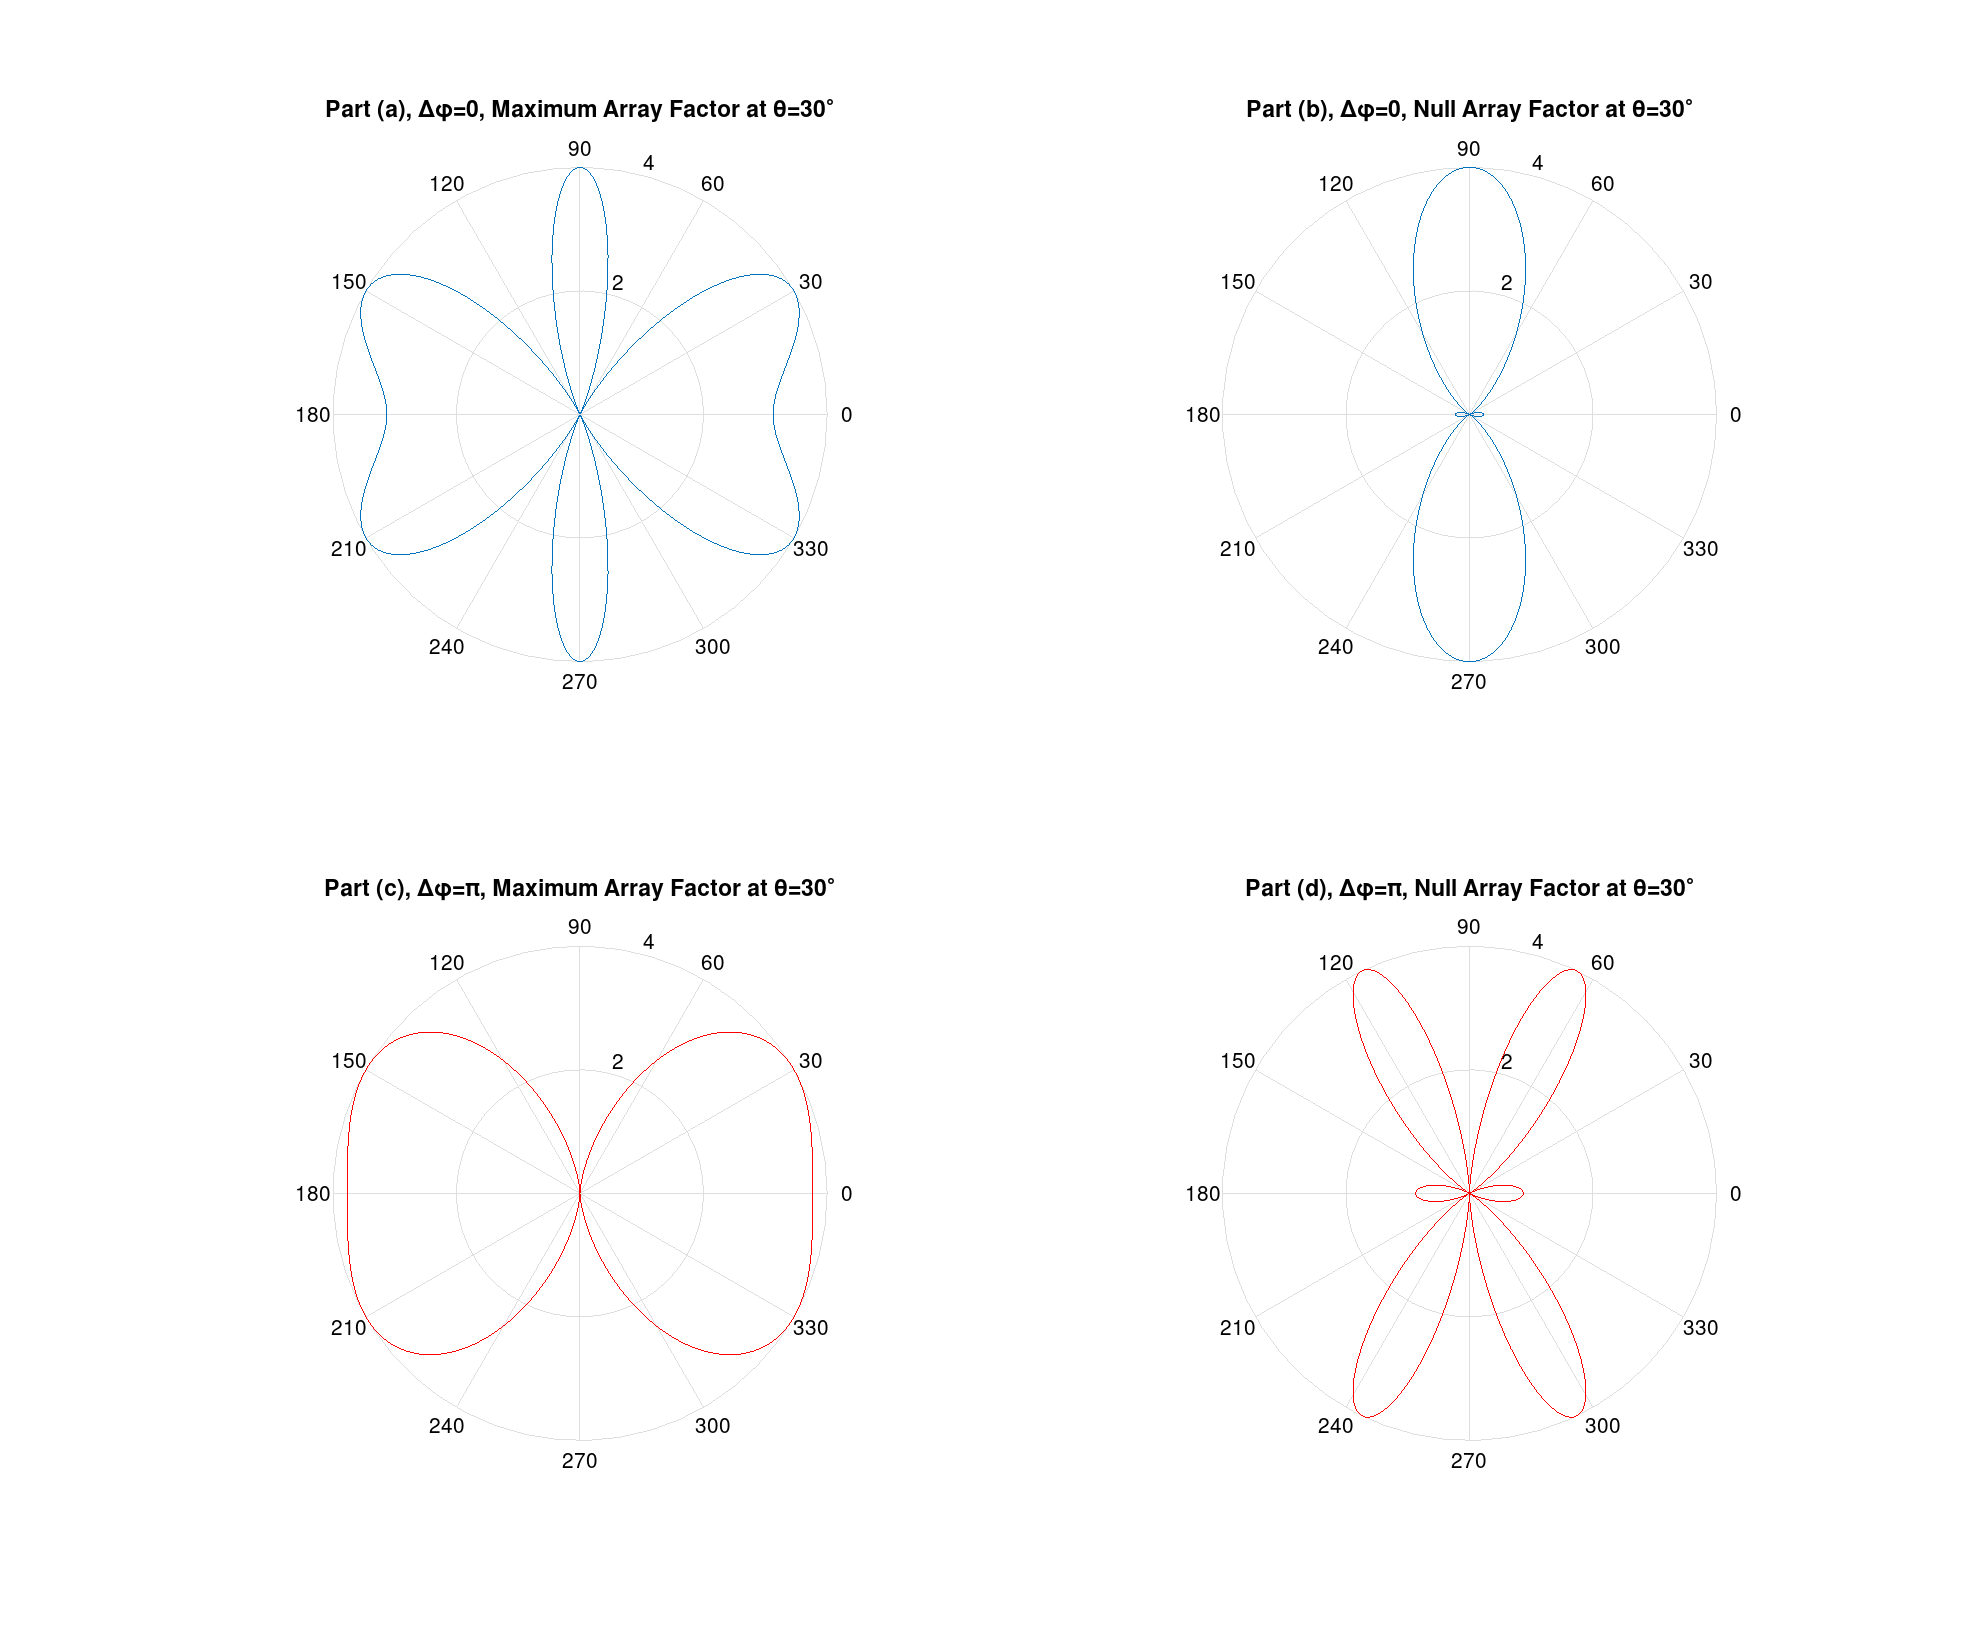
\includegraphics[width=.9\textwidth]{Figures/AFPlots.png}
          \caption{Plots of Array Factors}
          \label{fig:6}
        \end{figure}

        As expected, we can see plots 1 and 3 maximized at $30^{\circ}$ and plots 2 and 4 at 0.

    \end{enumerate}

  \item

    \begin{enumerate}

      \item 

        We can find the parallel polarization reflection coefficient using the formula:

        $$\Gamma_{\parallel}=\frac{\eta_2\cos(\theta_t)-\eta_1\cos(\theta_i)}{\eta_2\cos(\theta_i)+\eta_1\cos(\theta_i)}$$

        We can first find the transmitted angle using Snell's Law:

        $$n_1\sin(\theta_i)=n_2\sin(\theta_t)$$
        $$\theta_t=\sin^{-1}\left(\frac{n_1\sin(\theta_i)}{n_1}\right)$$
        $$\theta_t=\sin^{-1}\left(\frac{(1)\sin(50)}{\sqrt{4}}\right)$$
        $$\theta_t=22.52$$

        We apply this information to our formula:

        $$\Gamma_{\parallel}=\frac{\frac{1}{\sqrt{4}}\cos(22.52)-(1)\cos(50)}{\frac{1}{\sqrt{4}}\cos(22.52)+(1)\cos(50)}$$
        $$\boxed{\Gamma_{\parallel}=-.1638}$$


      \item 

        We know that the transmission coefficient is related to the reflection coefficient for parallel polarization by:

        $$\tau_{\parallel}=(1+\Gamma_{\parallel})\frac{\cos(\theta_i)}{\cos(\theta_t)}$$

        This gives us:

        $$\tau_{\parallel}=(1-.1638)\frac{\cos(50)}{\cos(22.52)}$$
        $$\boxed{\tau_{\parallel}=.5819}$$

      \item 

        For perpendicular polarization, we know that the reflection coefficient may be expressed as:

        $$\Gamma_{\perp}=\frac{\eta_2\cos(\theta_i)-\eta_1\cos(\theta_t)}{\eta_2\cos(\theta_i)+\eta_1\cos(\theta_t)}$$

        This yields:

        $$\Gamma_{\perp}=\frac{\frac{1}{2}\cos(50)-(1)\cos(22.52)}{\frac{1}{2}\cos(50)+(1)\cos(22.52)}$$
        $$\boxed{\Gamma_{\perp}=-.4838}$$

      \item 

        We know that the transmission coefficient relation to the perpendicular reflection coefficient is:

        $$\tau_{\perp}=(1+\Gamma_{\perp})$$

        This gives us:

        $$\tau_{\perp}=(1-.4838)$$
        $$\boxed{\tau_{\perp}=.5162}$$

      \item 

        The Brewster angle can be determined using:

        $$\theta_B=\tan^{-1}\left( \sqrt{\frac{\varepsilon_2}{\varepsilon_1}} \right)$$

        This gives us:

        $$\theta_{B\parallel}=\tan^{-1}\left( \sqrt{4} \right)$$
        $$\theta_{B\parallel}=\tan^{-1}\left( 2\right)$$
        $$\boxed{\theta_{B\parallel}=63.435^{\circ}}$$

      \item 

        We know that, for a nonmagnetic material (as the one described in the problem), the Brewster angle exists only for the parallel polarization (thus the use of $\theta_{B\parallel}$). A beam entering a medium at a this angle of incidence would fully transmit its parallel component (only the perpendicular component is reflected). This can be explained in the diagram below:

        \begin{figure}[H]
          \centering
          \tikzset{every picture/.style={line width=0.75pt}} %set default line width to 0.75pt        

\begin{tikzpicture}[x=0.75pt,y=0.75pt,yscale=-1,xscale=1]
%uncomment if require: \path (0,504); %set diagram left start at 0, and has height of 504

%Shape: Rectangle [id:dp24828463924463207] 
\draw  [color={rgb, 255:red, 80; green, 227; blue, 194 }  ,draw opacity=1 ][fill={rgb, 255:red, 80; green, 227; blue, 194 }  ,fill opacity=1 ] (138,229) -- (455,229) -- (455,333) -- (138,333) -- cycle ;
%Straight Lines [id:da47522454577861106] 
\draw    (171.5,128.79) -- (270.09,227.38) ;
\draw [shift={(271.5,228.79)}, rotate = 225] [color={rgb, 255:red, 0; green, 0; blue, 0 }  ][line width=0.75]    (10.93,-3.29) .. controls (6.95,-1.4) and (3.31,-0.3) .. (0,0) .. controls (3.31,0.3) and (6.95,1.4) .. (10.93,3.29)   ;
%Straight Lines [id:da1053230153406346] 
\draw    (271.5,228.79) -- (370.09,327.38) ;
\draw [shift={(371.5,328.79)}, rotate = 225] [color={rgb, 255:red, 0; green, 0; blue, 0 }  ][line width=0.75]    (10.93,-3.29) .. controls (6.95,-1.4) and (3.31,-0.3) .. (0,0) .. controls (3.31,0.3) and (6.95,1.4) .. (10.93,3.29)   ;
%Straight Lines [id:da4504340662665598] 
\draw    (271.5,228.79) -- (370.09,130.2) ;
\draw [shift={(371.5,128.79)}, rotate = 135] [color={rgb, 255:red, 0; green, 0; blue, 0 }  ][line width=0.75]    (10.93,-3.29) .. controls (6.95,-1.4) and (3.31,-0.3) .. (0,0) .. controls (3.31,0.3) and (6.95,1.4) .. (10.93,3.29)   ;

% Text Node
\draw (140,225.6) node [anchor=south west] [inner sep=0.75pt]    {$n_{1}$};
% Text Node
\draw (140,232.4) node [anchor=north west][inner sep=0.75pt]    {$n_{2}$};
% Text Node
\draw (169.5,125.39) node [anchor=south east] [inner sep=0.75pt]    {$( \perp ,\parallel )$};
% Text Node
\draw (373.5,125.39) node [anchor=south west] [inner sep=0.75pt]    {$( \Gamma_{\perp}\perp,0)$};
% Text Node
\draw (373.5,325.39) node [anchor=south west] [inner sep=0.75pt]    {$( \tau_{\perp}\perp , \parallel )$};


\end{tikzpicture}

          \caption{Brewster Angle Scenario}
          \label{fig:7}
        \end{figure}

        Given a coordinate set $(\perp,\parallel)$ representing each components strength, we can see that for the incident wave and transmitted wave, the perpendicular component experiences reflection. On the other hand, there is no parallel reflection.

      \item 

        We now assume that the same scenario occurs, but with the Brewster angle. This gives us:

        $$n_1\sin(\theta_i)=n_2\sin(\theta_t)$$
        $$\theta_t=\sin^{-1}\left(\frac{n_1\sin(\theta_i)}{n_2}\right)$$
        $$\theta_t=\sin^{-1}\left(\frac{\sin(63.435)}{2}\right)$$
        $$\boxed{\theta_t=26.565^{\circ}}$$

        From here, we can find the perpendicular reflection coefficient:

        $$\Gamma_{\perp}=\frac{\eta_2\cos(\theta_i)-\eta_1\cos(\theta_t)}{\eta_2\cos(\theta_i)+\eta_1\cos(\theta_t)}$$
        $$\Gamma_{\perp}=\frac{.5\cos(63.435)-\cos(26.565)}{.5\cos(63.435)+\cos(26.565)}$$
        $$\boxed{\Gamma_{\perp}=-.6}$$

        Note that the above result makes sense, as we expect the perpendicular component to be reflected. The parallel reflection becomes:

        $$\Gamma_{\parallel}=\frac{\eta_2\cos(\theta_t)-\eta_1\cos(\theta_i)}{\eta_2\cos(\theta_t)+\eta_1\cos(\theta_i)}$$
        $$\Gamma_{\parallel}=\frac{.5\cos(26.565)-\cos(63.435)}{.5\cos(26.565)+\cos(63.435)}$$
        $$\boxed{\Gamma_{\parallel}=0}$$

        The perpendicular transmission may be expressed as:

        $$\tau_{\perp}=(1+\Gamma_{\perp})$$
        $$\boxed{\tau_{\perp}=.4}$$

        Again, this makes sense as the perpendicular component will be reflected. The parallel transmission is:

        $$\tau_{\parallel}=(1+\Gamma_{\parallel})\frac{\cos(\theta_i)}{\cos(\theta_t)}$$
        $$\tau_{\parallel}=(1+0)\frac{\cos(63.435)}{\cos(26.565)}$$
        $$\boxed{\tau_{\parallel}=.5}$$

        \newpage

      \item 

        We can measure the Brewster angle using a similar lab set up to the one picture in \ref{fig:8} below:

        \begin{figure}[H]
          \centering
          \tikzset{every picture/.style={line width=0.75pt}} %set default line width to 0.75pt        

\begin{tikzpicture}[x=0.75pt,y=0.75pt,yscale=-1,xscale=1]
%uncomment if require: \path (0,504); %set diagram left start at 0, and has height of 504

%Shape: Can [id:dp24142366176937102] 
\draw  [fill={rgb, 255:red, 155; green, 155; blue, 155 }  ,fill opacity=1 ] (132.7,141) -- (55.3,141) .. controls (53.48,141) and (52,136.08) .. (52,130) .. controls (52,123.92) and (53.48,119) .. (55.3,119) -- (132.7,119) .. controls (134.52,119) and (136,123.92) .. (136,130) .. controls (136,136.08) and (134.52,141) .. (132.7,141) .. controls (130.88,141) and (129.4,136.08) .. (129.4,130) .. controls (129.4,123.92) and (130.88,119) .. (132.7,119) ;
%Shape: Can [id:dp6633481861245816] 
\draw  [fill={rgb, 255:red, 74; green, 74; blue, 74 }  ,fill opacity=1 ] (208.91,77.5) -- (231.31,77.5) .. controls (233.96,77.5) and (236.11,101.01) .. (236.11,130) .. controls (236.11,158.99) and (233.96,182.5) .. (231.31,182.5) -- (208.91,182.5) .. controls (206.26,182.5) and (204.11,158.99) .. (204.11,130) .. controls (204.11,101.01) and (206.26,77.5) .. (208.91,77.5) .. controls (211.56,77.5) and (213.71,101.01) .. (213.71,130) .. controls (213.71,158.99) and (211.56,182.5) .. (208.91,182.5) ;
%Shape: Ellipse [id:dp6329395443107491] 
\draw  [fill={rgb, 255:red, 74; green, 144; blue, 226 }  ,fill opacity=1 ] (204.11,130) .. controls (204.11,101.01) and (206.26,77.5) .. (208.91,77.5) .. controls (211.56,77.5) and (213.71,101.01) .. (213.71,130) .. controls (213.71,158.99) and (211.56,182.5) .. (208.91,182.5) .. controls (206.26,182.5) and (204.11,158.99) .. (204.11,130) -- cycle ;
%Straight Lines [id:da08647454737923055] 
\draw [color={rgb, 255:red, 208; green, 2; blue, 27 }  ,draw opacity=1 ]   (208.91,130) -- (133.4,130) ;
%Shape: Cube [id:dp5964729678243952] 
\draw  [fill={rgb, 255:red, 0; green, 0; blue, 0 }  ,fill opacity=1 ] (420.6,160) -- (414,153.4) -- (414,100) -- (429.4,100) -- (436,106.6) -- (436,160) -- cycle ; \draw   (414,100) -- (420.6,106.6) -- (420.6,160) ; \draw   (420.6,106.6) -- (436,106.6) ;
%Shape: Can [id:dp9110558709096379] 
\draw  [fill={rgb, 255:red, 74; green, 74; blue, 74 }  ,fill opacity=1 ] (311.62,77.5) -- (334.02,77.5) .. controls (336.67,77.5) and (338.82,101.01) .. (338.82,130) .. controls (338.82,158.99) and (336.67,182.5) .. (334.02,182.5) -- (311.62,182.5) .. controls (308.97,182.5) and (306.82,158.99) .. (306.82,130) .. controls (306.82,101.01) and (308.97,77.5) .. (311.62,77.5) .. controls (314.27,77.5) and (316.42,101.01) .. (316.42,130) .. controls (316.42,158.99) and (314.27,182.5) .. (311.62,182.5) ;
%Shape: Ellipse [id:dp3818053434961388] 
\draw  [fill={rgb, 255:red, 74; green, 144; blue, 226 }  ,fill opacity=1 ] (306.82,130) .. controls (306.82,101.01) and (308.97,77.5) .. (311.62,77.5) .. controls (314.27,77.5) and (316.42,101.01) .. (316.42,130) .. controls (316.42,158.99) and (314.27,182.5) .. (311.62,182.5) .. controls (308.97,182.5) and (306.82,158.99) .. (306.82,130) -- cycle ;
%Straight Lines [id:da010658672340027042] 
\draw [color={rgb, 255:red, 208; green, 2; blue, 27 }  ,draw opacity=1 ]   (311.62,130) -- (236.11,130) ;
%Straight Lines [id:da9472906998736996] 
\draw [color={rgb, 255:red, 208; green, 2; blue, 27 }  ,draw opacity=1 ]   (414.33,130) -- (338.82,130) ;

% Text Node
\draw (90.7,143) node [anchor=north] [inner sep=0.75pt]   [align=left] {Beam};
% Text Node
\draw (213.71,184) node [anchor=north] [inner sep=0.75pt]   [align=left] {\begin{minipage}[lt]{65.66pt}\setlength\topsep{0pt}
\begin{center}
Parallel\\Polarizer
\end{center}

\end{minipage}};
% Text Node
\draw (436,163) node [anchor=north] [inner sep=0.75pt]   [align=left] {Power Reader};
% Text Node
\draw (316.42,185) node [anchor=north] [inner sep=0.75pt]   [align=left] {\begin{minipage}[lt]{42.97pt}\setlength\topsep{0pt}
\begin{center}
Adjusted\\Polarizer
\end{center}

\end{minipage}};


\end{tikzpicture}

          \caption{Simplified Lab Set-up}
          \label{fig:8}
        \end{figure}

        A beam would be focused through a parallel polarizer and then a material with an adjustable angle (the ability to rotate to different angles). As this beam passes through the parallel polarizer,  only the parallel component will be passed through. The parallel-only beam would then pass through the adjustable material, and, subsequently, to the power reader. The power value is recorded with respect to the angle of the adjustable material, and then the angle of the material is modified (preferably in uniform steps). By definition, the transmitted parallel component of the beam would be maximized at the Brewster angle. Thus, as the power readings are taken, the Brewster angle is the angle that corresponds to the maximum power reading. 

    \end{enumerate}

  \item

    \begin{enumerate}

      \item 

        Given by the fact that field $\tilde{E}_i$ is directed in the $\bold{\hat{y}}$ direction, while being influenced by $x$ and $z$ components, we know that the wave is affected by \underline{perpendicular} polarization.

      \item 

        Given $3x+4z$, we may write:

        $$\theta_i=\tan^{-1}\left( \frac{3}{4} \right)$$
        $$\boxed{\theta_i=36.87^{\circ}}$$

      \item 

        This may be written in the time domain as:

        $$\tilde{E}_i=\bold{\hat{y}}20e^{-j(3x+4z)}$$
        $$E_i=20\cos(\omega t-(3x+4z))\bold{\hat{y}}$$

        We can find the angular frequency using the formula:

        $$\omega=ck$$

        This gives us:

        $$\omega=c\sqrt{3^2+4^2}$$
        $$\omega=5c$$
        $$\omega=1.5\cdot10^{9}\left[ \frac{\text{rad}}{\si{\second}} \right]$$

        Thus, we get:

        $$\boxed{E_i=20\cos((1.5\cdot10^9) t-(3x+4z))\bold{\hat{y}}}$$

      \item 

        The average power density is defined by the formula:

        $$S_{avg}=\frac{|E|^2}{2\eta}$$

        Since the incident wave is traveling in air, we may write:

        $$\eta=\eta_o=376.819[\si{\ohm}]$$

        Since, from the time domain, we know the magnitude of the wave, we may write:

        $$S_{avg}=\frac{(20)^2}{2\cdot376.819}$$
        $$\boxed{S_{avg}=.531\left[ \frac{\si{\watt}}{\si{\meter\squared}} \right]}$$

      \item 

        Since the wave is perpendicularly polarized, know that the magnitude of the reflected wave can be defined using:

        $$|E^r|=\Gamma|E^i|$$

        The reflection coefficient may be defined as:

        $$\Gamma_{\perp}=\frac{\eta_2\cos(\theta_i)-\eta_1\cos(\theta_t)}{\eta_2\cos(\theta_i)+\eta_1\cos(\theta_t)}$$

        Now, we need to find the transmitted angle:

        $$\theta_t=\sin^{-1}\left( \frac{n_1\sin(\theta_i)}{n_2} \right)$$
        $$\theta_t=\sin^{-1}\left( \frac{\sin(36.87)}{2} \right)$$
        $$\theta_t=17.48^{\circ}$$

        From here, we return to the reflection coefficient:

        $$\Gamma_{\perp}=\frac{.5\cos(36.87)-\cos(17.48)}{.5\cos(36.87)+\cos(17.48)}$$
        $$\Gamma_{\perp}=-.409$$

        This means that the magnitude becomes:

        $$|E^r|=|-.409\cdot20|=8.18$$

        This gives us:

        $$S_{avg}=\frac{|8.18|^2}{2\cdot376.819}$$
        $$\boxed{S_{avg}=.0888\left[ \frac{\si{\watt}}{\si{\meter\squared}} \right]}$$

    \end{enumerate}

\end{enumerate}

\end{document}

